\documentclass{NSF}

\graphicspath{{figures/}}

\usepackage{amsmath}
\usepackage{amssymb}

\usepackage{listings}
\usepackage{fancybox}
\usepackage{tikz}
\usepackage{enumitem}
\usepackage{multicol}

\newtheorem{mydef}{Definition}

\graphicspath{{figures/}}

\begin{document}

% A. Cover Sheet
% A number of the boxes contained on the Cover Sheet are
% electronically pre-filled as part of the FastLane login process
% Complete the rest of your info there

\pagestyle{headings}
\markright{}

% B. Project Summary
\title{Unsupervised Gaussian embedding matching \\ using normalising flows}
\section{Proposal for Master Thesis Project}

\subsection{Motivation}

Close to 1. mio. people immigrated to Europe in the year of 2015.
This proposes difficulties to local labour markets, where jobs from the origin-country do not entail the same meaning as jobs in the new host country.
Being a fisher in Syria or Turkey includes a different set of skills from being a fisher in Germany, as the same occupation in different countries have different underlying skillsets (and thus a different meaning). \\
A similar problem arises in the context of NLP.
When applying bilingual lexicon induction, words in language A do not carry a one-to-one correspondence in language B, although it is obvious that up to some uncertainty, a (bijective) mapping between tokens are possible.

\subsection{Background}

The above two problems can be regarded as finding an invertible transformation from one (embedding) space $\mathcal{X} \in \mathbf{R}^d$ into another $\mathcal{\hat{X}} \in \mathbf{R}^d$.
Normalised flows have proven to be a powerful tool in modeling such relations.
As such, the aim of this project is to find a model based on normalising flows which is able to find an an invertible mapping $f$ from $\mathcal{X}$ to $\mathcal{\hat{X}}$.
To keep the discussion focused, this thesis work deals with the problem of finding a model for bilingual lexicon matching.

\subsubsection{Gaussian Embeddings}
Gaussian embedding \cite{gaussian_embedding} is a set of probability distributions which embed tokens $ v_i = \mathcal{N}(x; \mu_i, \Sigma_i) $ as Gaussian distributions in the latent embedding space with learnable parameters $\theta = [\mu_i, \Sigma_i]$.
This is in contrast to the more commonly used vector-embeddings, as proposed by word2vec \cite{wordvec} or GloVe \cite{pennington2014glove}, where the learned embedding is merely a vector $v_i \in \mathcal{R}^d$.
The Gaussian embeddings $v_i$ are more robust, but also more difficult to train.

\subsubsection{Normalising Flows}

Normalising flows \cite{variational_inference_using_normalized_flows}, \cite{normalising_flows} is a powerful framework for building powerful posteriors through an iterative procedure.
We start with a simple distribution , and apply a set of invertible transformations transformations $f_t$, s.t. the last iterate $z^T$ has a more flexible / powerful distribution.
Specifically (for finite normalising flows), $z_0 \sim q_0(z_0|x)$ and $z_t = f_t(z_{t-1}, x)$.
As long as we have access to a jacobian of the transforming bijection, the probability density function of the last iterate can be computed.
These can be used for classification and clustering \cite{normalising_flows},  variational inference tasks \cite{iaf} such as image-generation \cite{nvp}.

\subsubsection{Unsupervised bilingual lexicon matching}

Bilingual lexicon matching is the task of finding a target token in language B, a corresponding source token in language A.
More generally, this can be seen as translating one vector-space into another, addressing the need for a common embedding space amongst items \cite{wordvec}, \cite{nmtrepresentation}.
Existing work includes cross-domain audio/text/image generation \cite{microsoft_3way} \cite{syd_gan} \cite{conditional_image_to_image} \cite{bair_gan}, and also unsupervised language translation \cite{unsupervised_phrasebased_translation}.
There has also been some work in matching tokens of a source language with bilingual lexicon matching \cite{art_1} \cite{art_2}, \cite{springer}.
Unsupervised methods aim at minimizing a global cosine error between the two embedding spaces \cite{muse}.

\subsection{Scope of Work}

Normalising flows are a powerful tool for finding an invertible map from one (usually simple) probability density to another.
Bilingual lexicon matching considers the problem of finding a target token in language B for each source token in language A.
We now adopt the observation made in \cite{density_matching}, and look at the embedding space not as a space of point-vectors, but as a high-dimensional, complex probability distributions.
Continuing where \cite{density_matching} left off, we want to investigate the performance of using normalising flows to model unsupervised lexicon matching between two probability distributions, which are defined by Gaussian emebddings, which have a one-to-one correspondence to tokens in the respective languages.
We aim to use Gaussian embeddings for the robustness, and better integration into the probabilistic perspective.
The Gaussian embedding space can be interpreted as a high-dimensional GMM model, where we have one Gaussian distribution for each word present. \\

We propose following steps on achieving this goal

\begin{enumerate}[topsep=2pt, partopsep=2pt]
    \item Replicate the algorithms and models which can generate through Gaussian embedding. Do one sanity check by doing a sanity check on one of (SimLex / WordSim)
    \item Replicate "Density matching for bilingual word embedding" to setup a baseline normalising flow between vector-word-embeddings \cite{density_matching}
    \item Define loss between predicted and target embeddings (if change in definition is necessary)
    \item Change the embeddings in point 2. to use Gaussian embeddings. Implement Loss functions found in point 3.
\end{enumerate} \\

If the above points provide good performance , we would like to expand on the below points.

\begin{enumerate}
    \item Investigate "deeper" normalising flows than the linear flow in \cite{density_matching} as such.
    \item Use other embedding-distributions for the word-embeddings (i.e. Dirichlet)
\end{enumerate}\\

As a contingency plan (but also if more time allows for next steps), implementing the following points would allow for an applied perspective of this approach, showing that this methodology allows for more robust mapping, also outside the field of NLP.

\begin{enumerate}
    \item Train embeddings for job-systems ESCO and AUGOV using Skip-Gram or Co-Occurence-matrix based. Do a sanity check.
    \item Train Gaussian embeddings for job-systems. Do a sanity check.
    \item Generate a small validation dataset between the European job-system and Australian job-system.
    \item Setup some baseline algorithms based on NLP, graph-matching, colinear-PCA for matching as a non-NLP benchmark environment. Compare against above-proposed methods.
    \item Find a normlising flow model to transform one job system into another.
    \item Build two transformation functions, (examplified by cycle-GANs)
\end{enumerate}


% E. References Cited
\renewcommand\refname{References}
\bibliography{references}
% I prefer to use the IEEE bibliography style.
% That's  NOT required by the NSF guidelines.
% Feel Free to use whatever style you prefer
\bibliographystyle{IEEEtran}

\newpage
\section{Appendix A}

\subsubsection{Further applications}

\begin{figure}[hb]{0.6\textwidth}
  \centering
  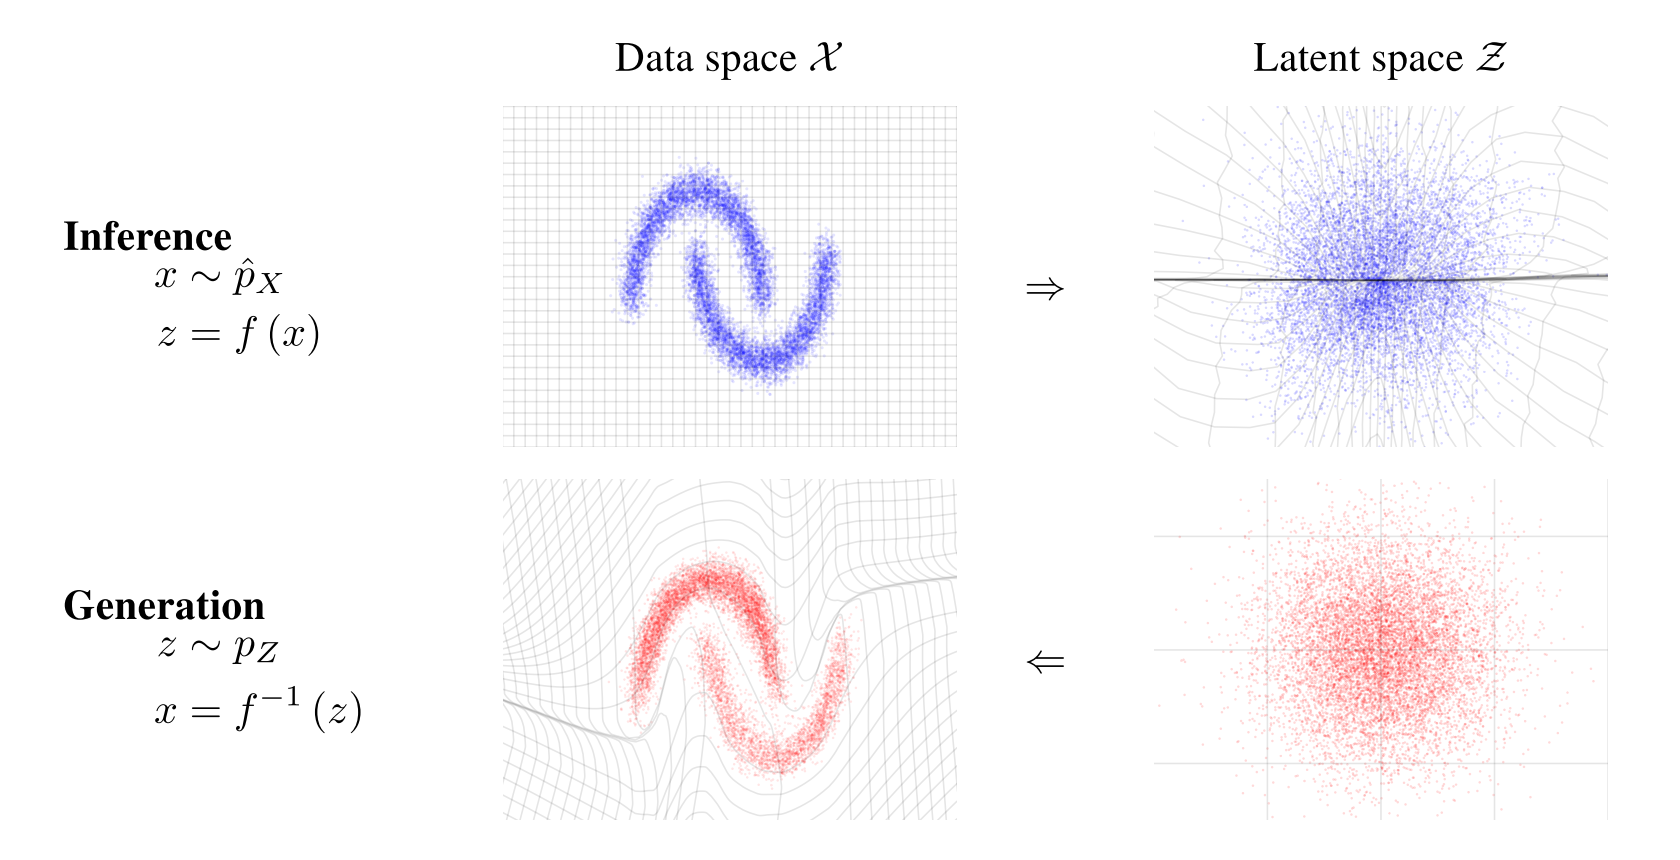
\includegraphics[width=10cm]{NVP.png}
  \caption{Figure from \cite{nvp}. Real-valued, non-volume-preserving density estimation, uses normalising flows to find an invertible mapping from one probability distribution to another.}
  \label{fig:test}
\end{figure}

However, in many real-world applications desire a single universal latent space which is valid amongst all latent vectors.
One way to achieve this is by translating one such latent space into another, allowing for different concepts to live in the same vector-space.

[BS]
Thinking further, the abstratization of embedding matching can be used by collaborative filtering methods to apply domain adaption to unseen domains, which already have a non-overlapping userbase as the current dataset.
Specifically, if we have users $\mathcal{X}$ and users $\mathcal{\hat{X}}$, who have respectively watched movies $\mathcal{A}$ and users $\mathcal{\hat{A}}$, we can now find a mapping $f: \mathcal{X} \Longrightarrow \mathcal{\hat{X}}$, and improve recommendations for both user-bases (due to the increased size of the dataset).
For this, of course, the mapping needs to be robust enough, or better-performing relative to the recommendation algorithm. \\

Some "naive" techniques to map one job-system into another include co-linear PCA models, NLP-based techniques (tf-idf, BERT, etc.) as well as the Google Knowledge Graph.

\subsubsection{Further Motivation behind using Normalising Flows}

An empirical loss function which is often maximized is the ELBO, which arises through the below maximization of the log-probability.

\begin{align*}
    log p_{\theta}(\mathbf{x}) &= \log \int p_{\theta}(\mathbf{x} | \mathbf{z}) p(\mathbf{z}) d \mathbf{z} \\
&=\log \int \frac{q_{\phi}(\mathbf{z} | \mathbf{x})}{q_{\phi}(\mathbf{z} | \mathbf{x})} p_{\theta}(\mathbf{x} | \mathbf{z}) p(\mathbf{z}) d \mathbf{z} \\ &\geq-\mathbb{D}_{\mathrm{KL}}\left[q_{\phi}(\mathbf{z} | \mathbf{x}) \| p(\mathbf{z})\right]+\mathbb{E}_{q}\left[\log p_{\theta}(\mathbf{x} | \mathbf{z})\right]
\end{align*}

Here, the first term acts as a regularizer (target distribution should match sampling-distribution), and the second term maximizes the "naive" match of the datapoints.

The sample-distribution $q$ should be chosen in such a way that the true data-distribution can be modeled.
As proposed in \cite{variational_inference_using_normalized_flows}, an ideal family of variational distributions $q_\phi(z|x)$ is one that is highly preferable, which could possibly also include the true posterior as a solution.
Due to their high expressivity, normalising flows also provide to be a good family of functions to model such a distribution.
The problem of picking this distribution falls aways.
However, the problem of transforming the existing distribution into another (often simpler) distribution arises.
Given the recent success, this problem seems to be an easier one to solve in certain applications.

[BS]
We can use neural networks to emulate such a sequential, volume-preserving transformation on the initial probability distribution.
Each individual component is then expressed through \textit{change of variable formula} for probability distributions \cite{nvp}.

\begin{equation}
    p_X(x) = p_Z(z) | \text{det} \left( \frac{ \delta g(z) }{ \delta z^T} \right) |^{-1}
\end{equation}

which stands in similarity to changing one probability density into another.

\begin{equation}
    \rho(x) = J(x) \mu( y(x) )
\end{equation}

as described in \cite{normalising_flows_classification_clustering}.

In addition to that, one can exploit additional useful properties through the overlapping probability density distribution to encode inherent structure in the joint probability models.
However, Gaussian embeddings are more difficult to train due to the energy-based loss functions and training.

\end{document}